\chapter{lecturePresenter}

\section{Vorbereitung}
Stellen Sie sicher, dass \lectStudio{} auf ihrem Gerät installiert ist. Anweisungen für die Installation finden Sie in Abschnitt \ref{section:installation} dieses Dokuments.
\\\\
Erstellen Sie die Vorlesungsfolien in einem Programm ihrer Wahl. Um sie in \lectStudio{} verwenden zu können, müssen Sie die Folien als PDF exportieren. Es wird empfohlen, die Folien mit dem gleichen Seitenverhältnis anzulegen, mit dem sie auch präsentiert werden sollen.

\subsection*{PowerPoint-Präsentation in ein PDF umwandeln}
Sollten Sie ihre Präsentation mit PowerPoint erstellt haben, dann haben Sie mehrere Möglichkeiten die PowerPoint-Folien in ein PDF umzuwandeln.

Hat ihre Präsentation einfache Animationen, dann bietet sich das Werkzeug \textbf{\href{http://www.maxonthenet.altervista.org/ppsplit.php}{PPspliT}} an. Dazu laden und installieren Sie die neueste Version von PPspliT. Um das Werkzeug zu verwenden, öffnen Sie die Präsentation mit PowerPoint und suchen in der Menü-Leiste nach \quote{PPspliT} (\autoref{fig:ppsplit}).

\begin{figure}[H]
	\centering
	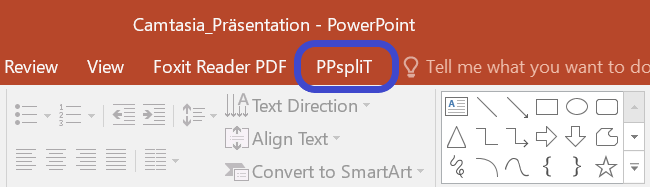
\includegraphics[width=0.57\textwidth]{presenter/ppsplit}
	\caption{PowerPoint-Präsentation mit PPspliT in PDF umwandeln}
	\label{fig:ppsplit}
\end{figure}

Sollten Sie kein PowerPoint haben, dann können Sie ihre Präsentation mit \textbf{\href{https://de.libreoffice.org/download/download/}{LibreOffice}} in ein PDF umwandeln. Laden und installieren Sie hierzu die neueste Version von LibreOffice. Als nächstes öffnen Sie die Präsentation mit LibreOffice und wandeln diese über das Menü \menu[,]{Datei, Als PDF exportieren} in PDF um.


\subsection*{Digitale Stifteingabe}
\lectPresenter{} ist mit dem Ziel entwickelt worden, um mit einem digitalen Stift zu arbeiten. Die digitale Stifteingabe ist zum Beispiel mit Convertibles wie Microsoft Surface Pro oder Lenovo Yoga möglich. Es ist auch möglich ein zum PC zusätzliches Tablet wie \href{https://www.huion.com/pen_display}{HUION Kamvas} mit Stift zu verwenden.


\subsection*{Vor der Präsentation}

\subsubsection{Mikrofon}
Schließen Sie das zu verwendende Mikrofon an den Rechner an. Sie können ein externes Headset benutzen, oder -- sofern vorhanden -- die Hörsaal-Audio-Anlage mit dem Laptop verbinden.
Viele Laptops besitzen auch ein eingebautes Mikrofon, es wird jedoch von seiner Verwendung abgeraten, da die Audioqualität für gewöhnlich zu wünschen übrig lässt -- besonders, wenn sich der Vortragende vom Rechner entfernt.
\\
Richten Sie nun das gewünschte Mikrofon ein (\autoref{fig:presenter-audio-settings}):
\begin{enumerate}
	\item Öffnen Sie die Einstellungen \menu[,]{Bearbeiten, Einstellungen}.
	\item Navigieren Sie zum Tab \textbf{Mikrofon}.
	\item Wählen Sie das korrekte Mikrofon aus [1].
	\item Mit dem Regler [2] können Sie die Lautstärke des Mikrofons anpassen.
	\item Alternativ können Sie die Aufnahmelautstärke anpassen, indem Sie den Aufnahmepegel automatisch einstellen lassen [3].
	
	Klicken Sie im Dialog (\autoref{fig:presenter-audio-settings-auto}) auf \textbf{Beginnen} und sprechen Sie eine Zeit lang in das ausgewählte Mikrofon. Nachdem Sie auf \textbf{Fertig} gecklickt haben, wird die Mikrofonlautstärke auf den maximal erreichten Pegel eingestellt.

	\item Machen Sie eine kurze Aufzeichnung [4] und überprüfen diese auf Rauschen, Nebengeräusche, Hall, usw.
	\item Abschließend klicken Sie auf den Button \textbf{Schließen}, um die Einstellungen zu speichern.
\end{enumerate}

\begin{figure}[H]
	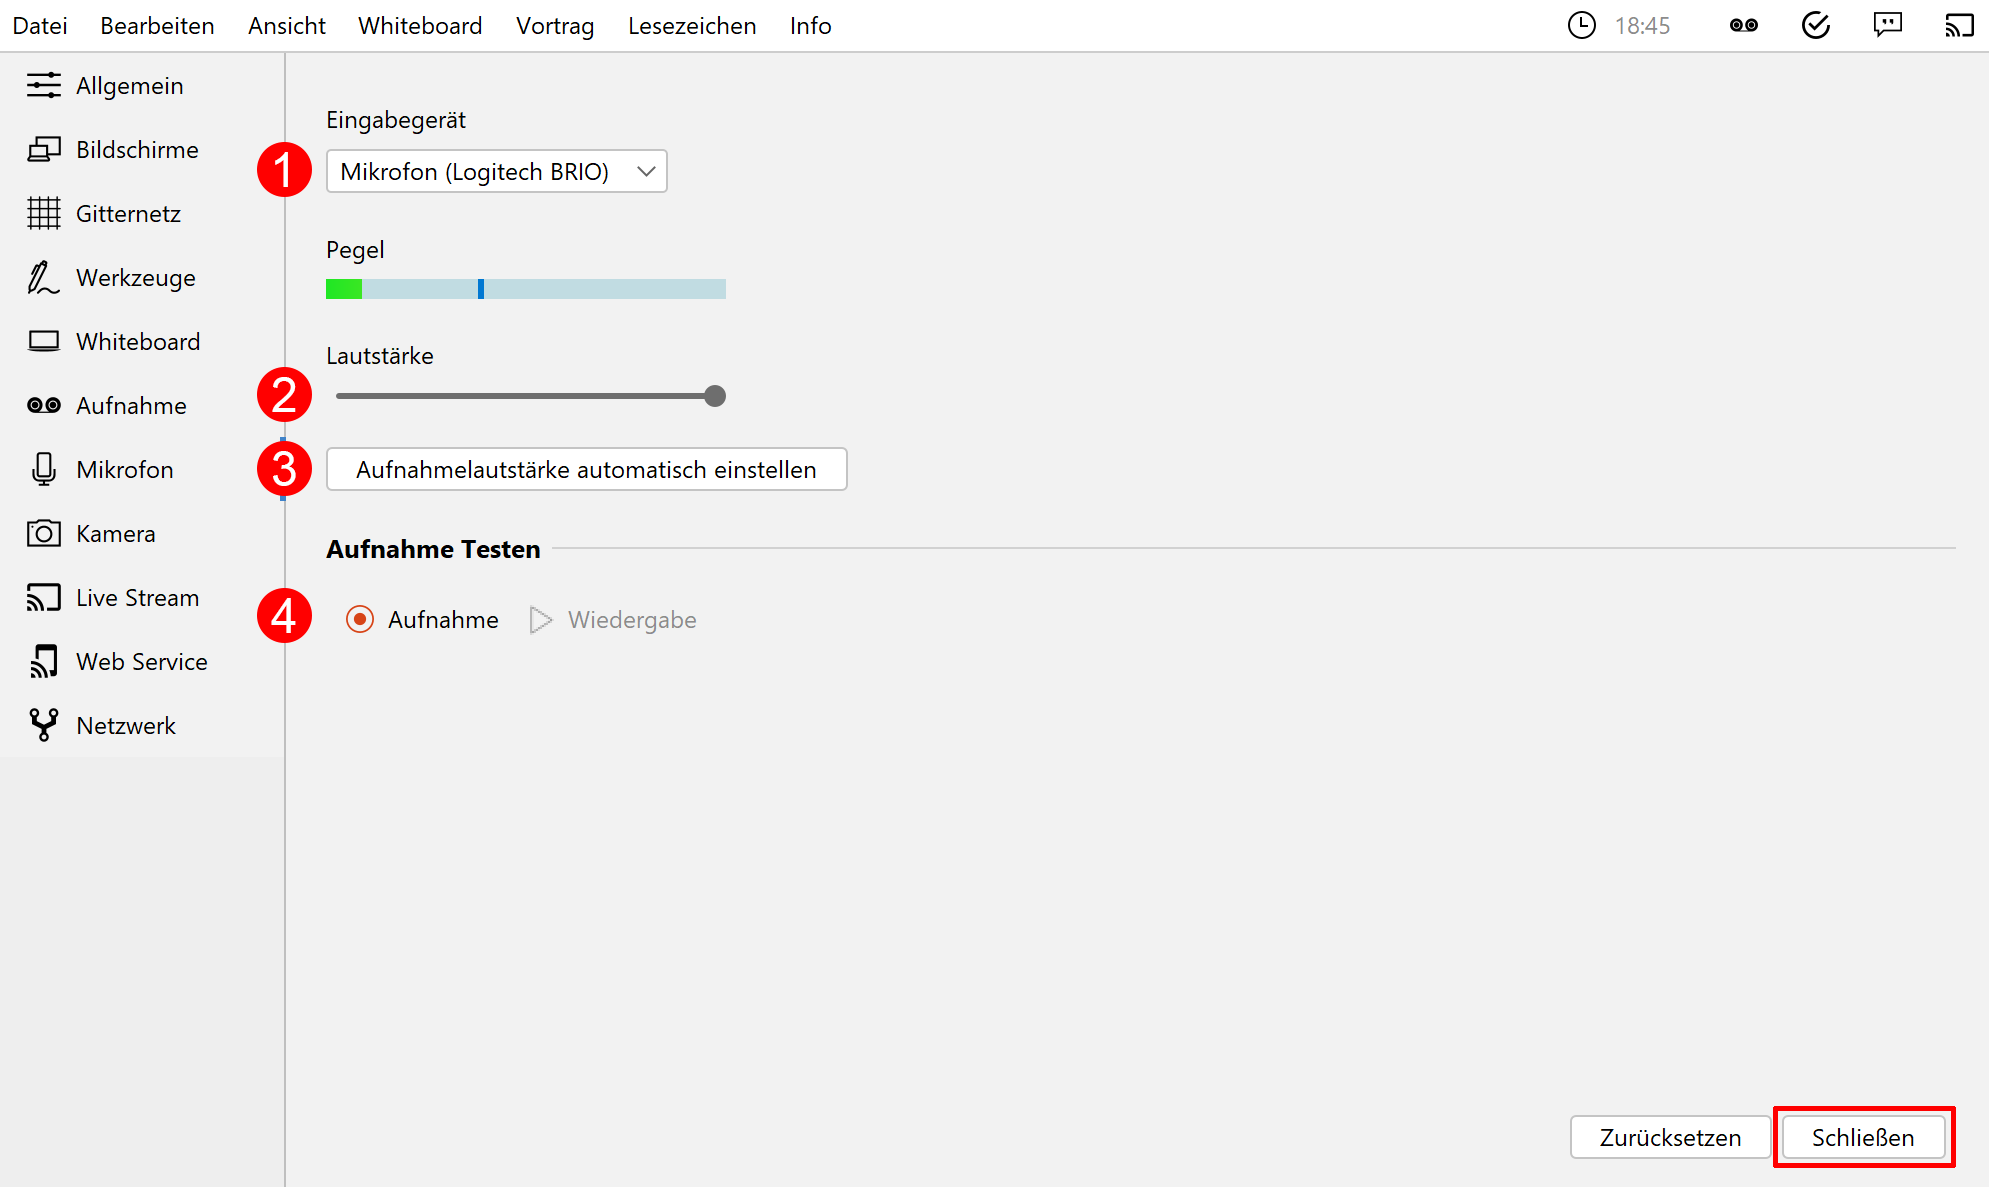
\includegraphics[width=\textwidth]{presenter/audio-settings}
	\caption{Mikrofon-Einstellungen}
	\label{fig:presenter-audio-settings}
\end{figure}
\begin{figure}[H]
	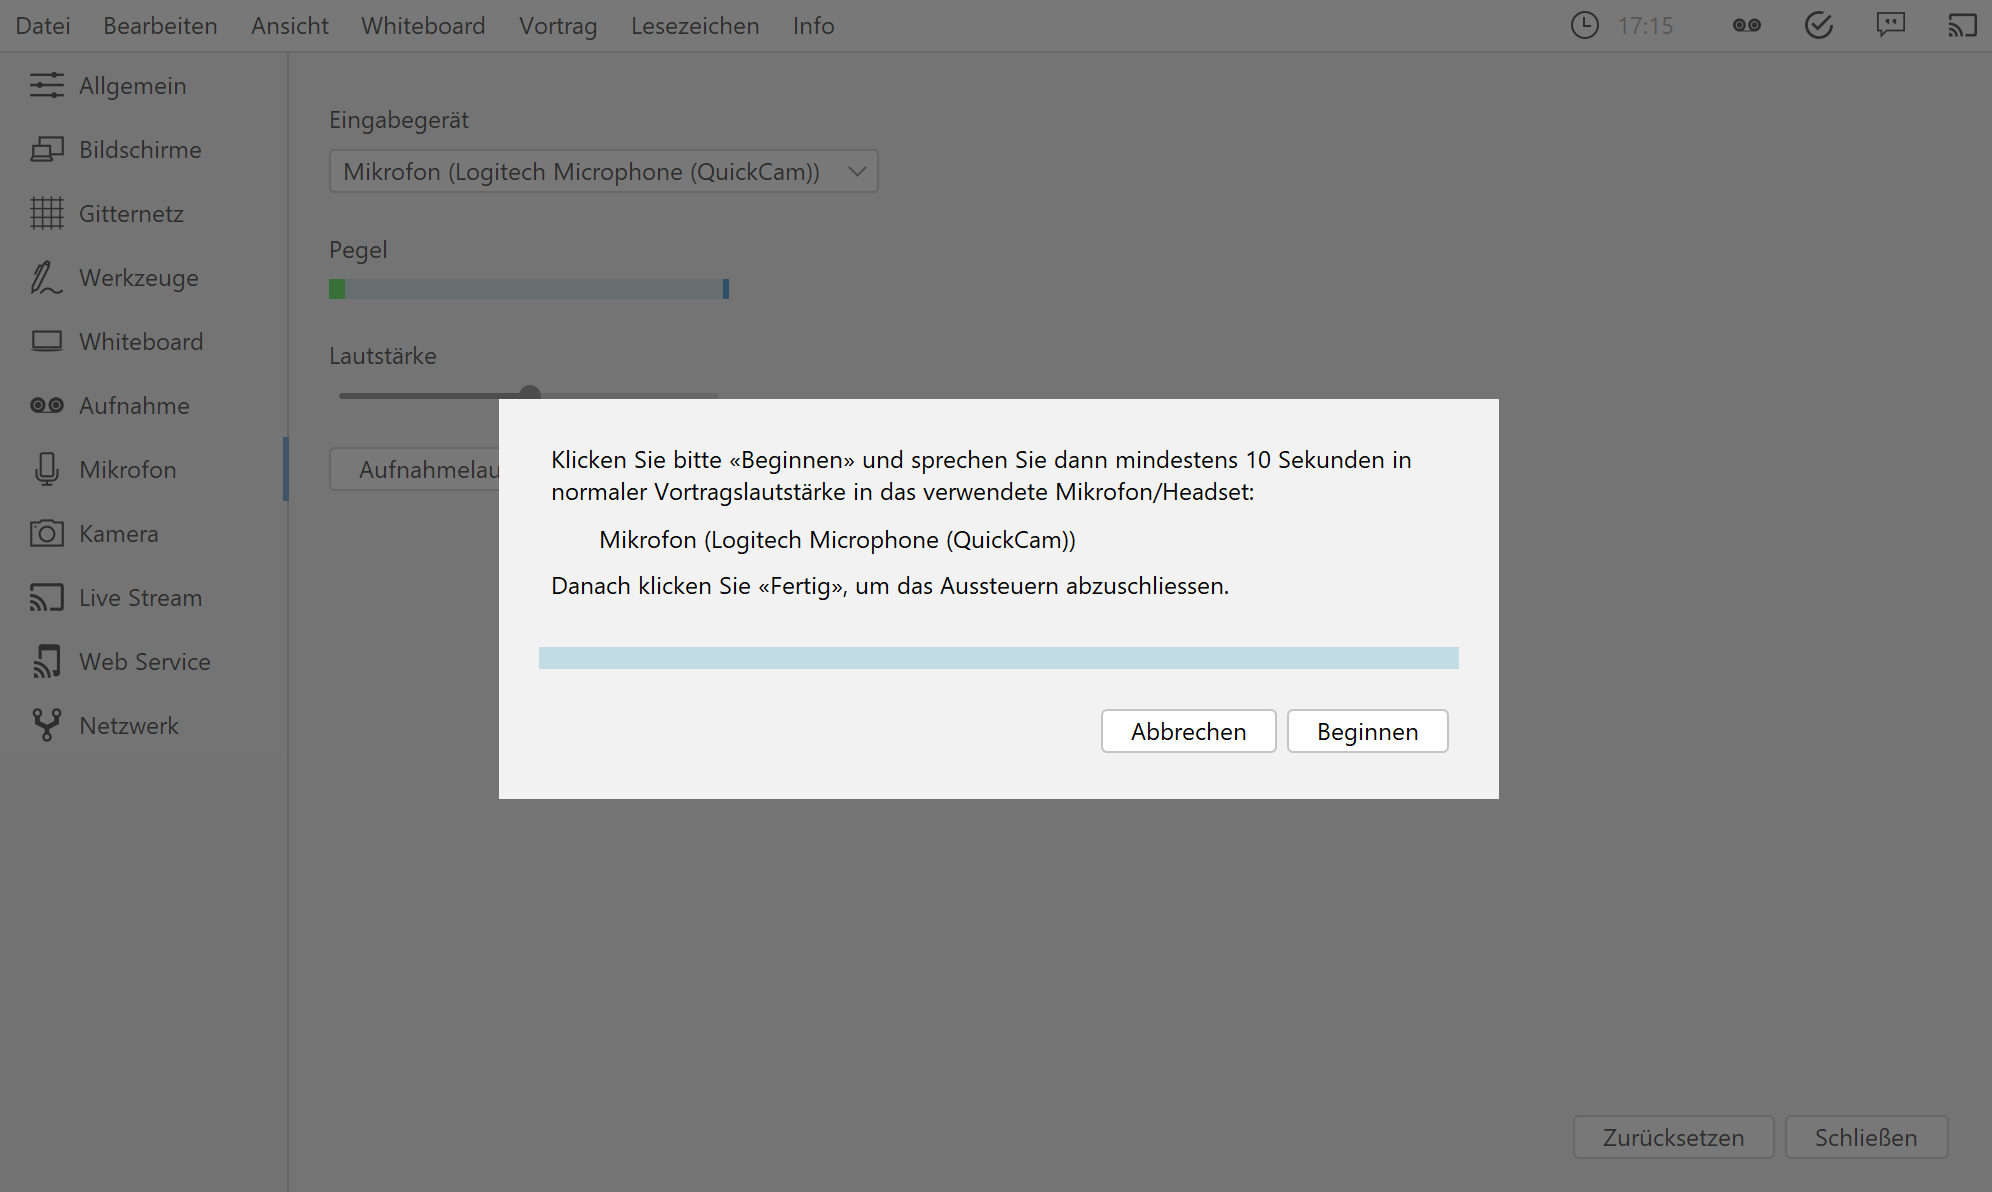
\includegraphics[width=\textwidth]{presenter/audio-settings-auto}
	\caption{Aufnahmepegel automatisch einstellen}
	\label{fig:presenter-audio-settings-auto}
\end{figure}

\subsubsection{Anzeigegeräte}
Verbinden Sie den Videoausgang des Rechners mit dem Eingang des Anzeigegerätes, und vergewissern Sie sich, dass das Anzeigegerät eingeschaltet ist.
\\\\
Sie können den aktuellen Projektionsmodus einsehen und ändern:
\begin{itemize}
	\item \textbf{Windows}\par
	Mit der Tastenkombination \keys{\faWindows{} + \textbf{P}} die Projektions-Seitenleiste öffnen.
	\begin{note}
		Achten Sie darauf, dass der Projektionsmodus auf \quote{\textbf{Erweitern}} gestellt ist, \textbf{nicht} auf \quote{Duplizieren}.
	\end{note}

	\item \textbf{Linux (Ubuntu)}\par
	Öffnen Sie die \textbf{Aktivitäten}-Übersicht und tippen \quote{Anzeige} ein, danach klicken Sie auf \quote{Anzeigegeräte}.
	\begin{note}
		Achten Sie darauf, dass in der Bildschirmkonfiguration die Option \quote{Bildschirm spiegeln} \textbf{nicht} ausgewählt ist.
	\end{note}
	\begin{info}
		Diese Schritte können sich in anderen Linux-Distributionen unterscheiden.
	\end{info}

	\item \textbf{macOS}\par
	Über das Apple-Menü \menu[,]{\faApple, Systemeinstellungen}, und auf \quote{Displays} klicken.
	\begin{note}
		Achten Sie darauf, dass das Markierungsfeld \quote{Bildschirme synchronisieren} \textbf{nicht} aktiviert ist.
	\end{note}
\end{itemize}

Aktivieren Sie die Ausgabe der Folien auf dem Projektor (\autoref{fig:presenter-toolbar}, Markierung 21).


\section{Grundlagen des Arbeitsbereichs}

Starten Sie \lectPresenter{} über das Startmenü oder den Desktop Shortcut. Sie werden dann mit dem Startbildschirm begrüßt. Hier können Sie entweder eine der zuletzt geöffneten Dateien laden, ein leeres Whiteboard öffnen, oder über den Button \quote{Dokument öffnen} eine neue Datei auswählen.

\begin{figure}[H]
	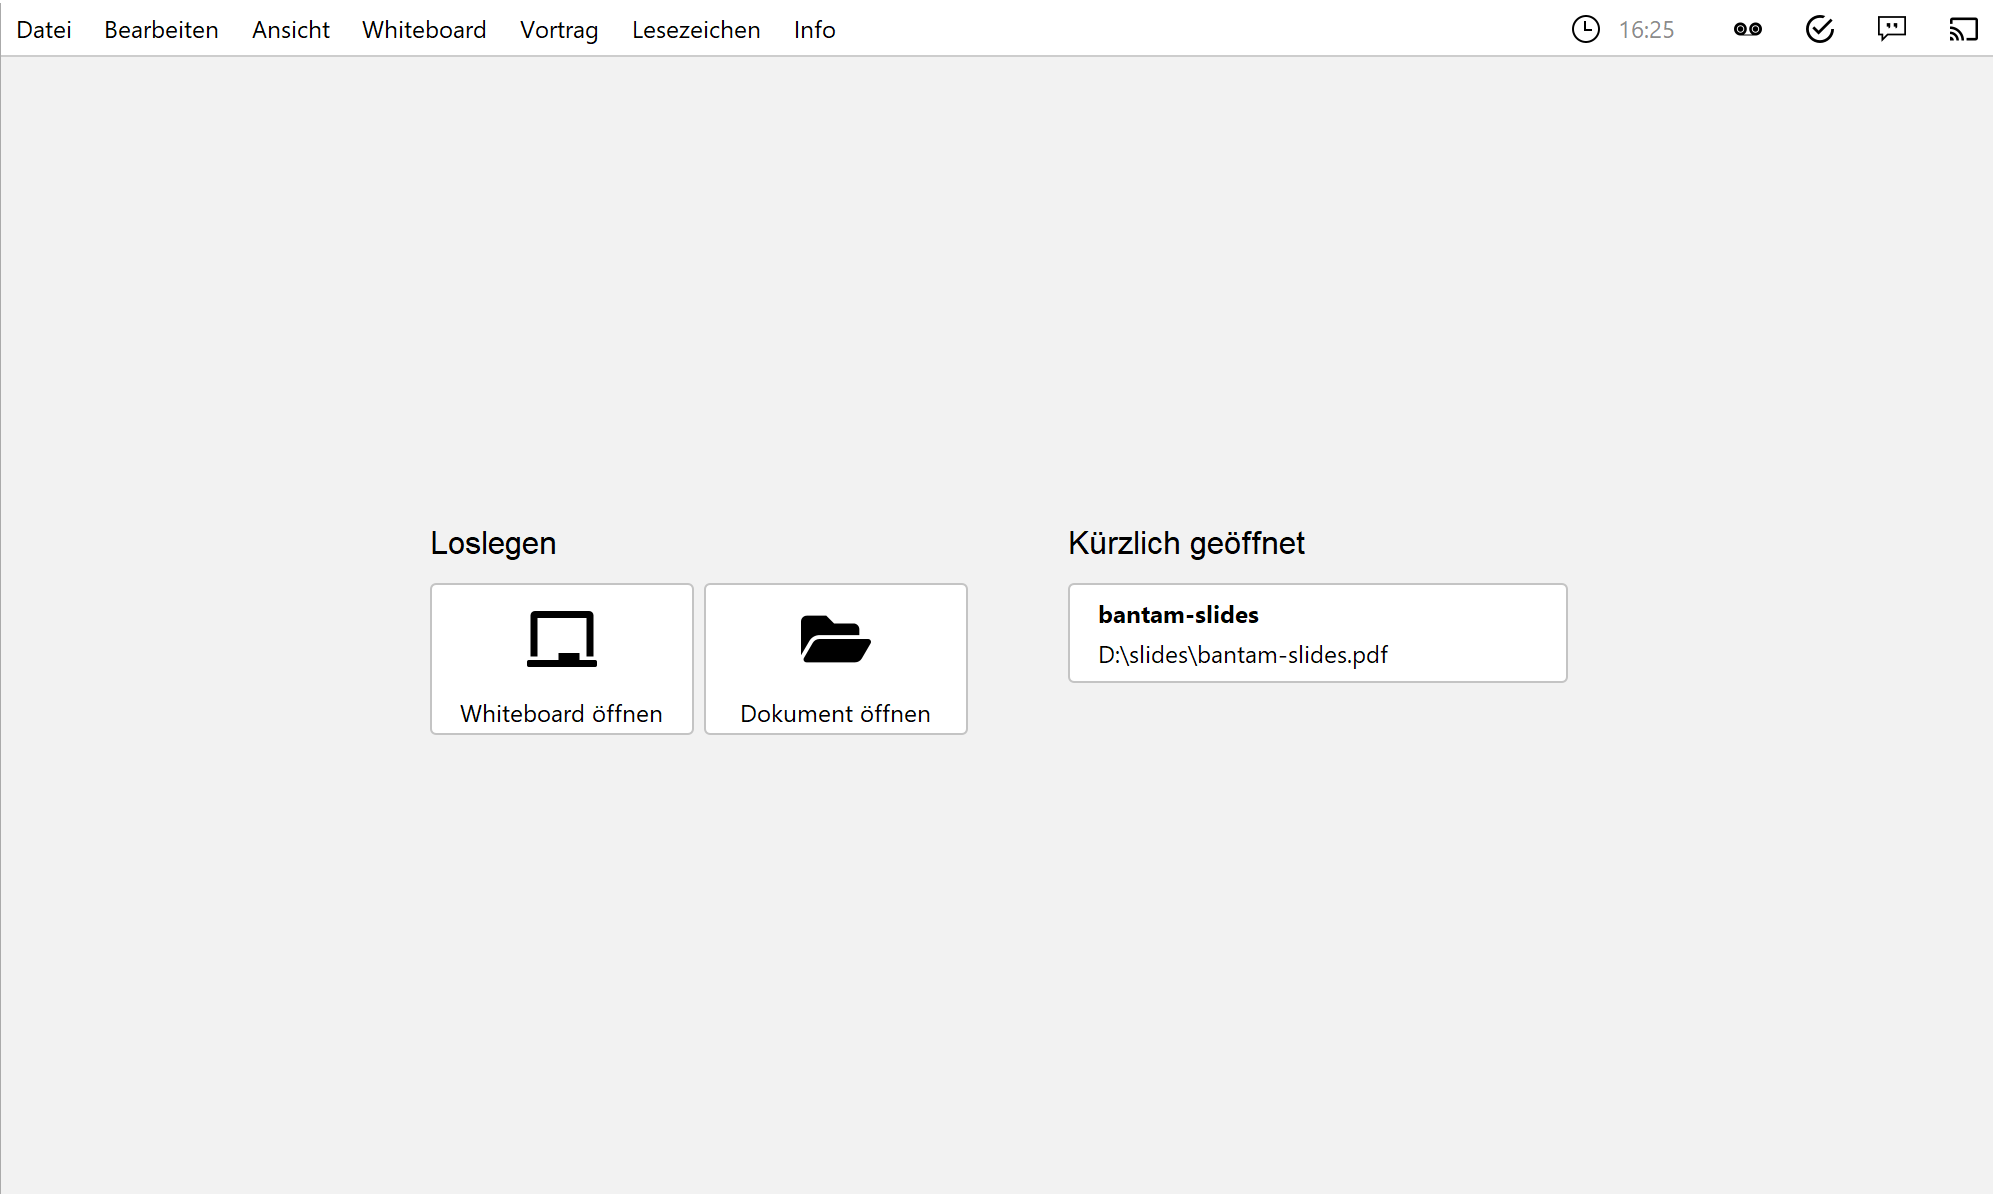
\includegraphics[width=\textwidth]{presenter/start}
	\caption{Startbildschirm}
	\label{fig:presenter-start}
\end{figure}

Sobald Sie ein PDF-Dokument oder ein Whiteboard geöffnet haben, finden Sie die Benutzeroberfläche wie in \autoref{fig:presenter-overview} dargestellt wieder.

\begin{figure}[H]
	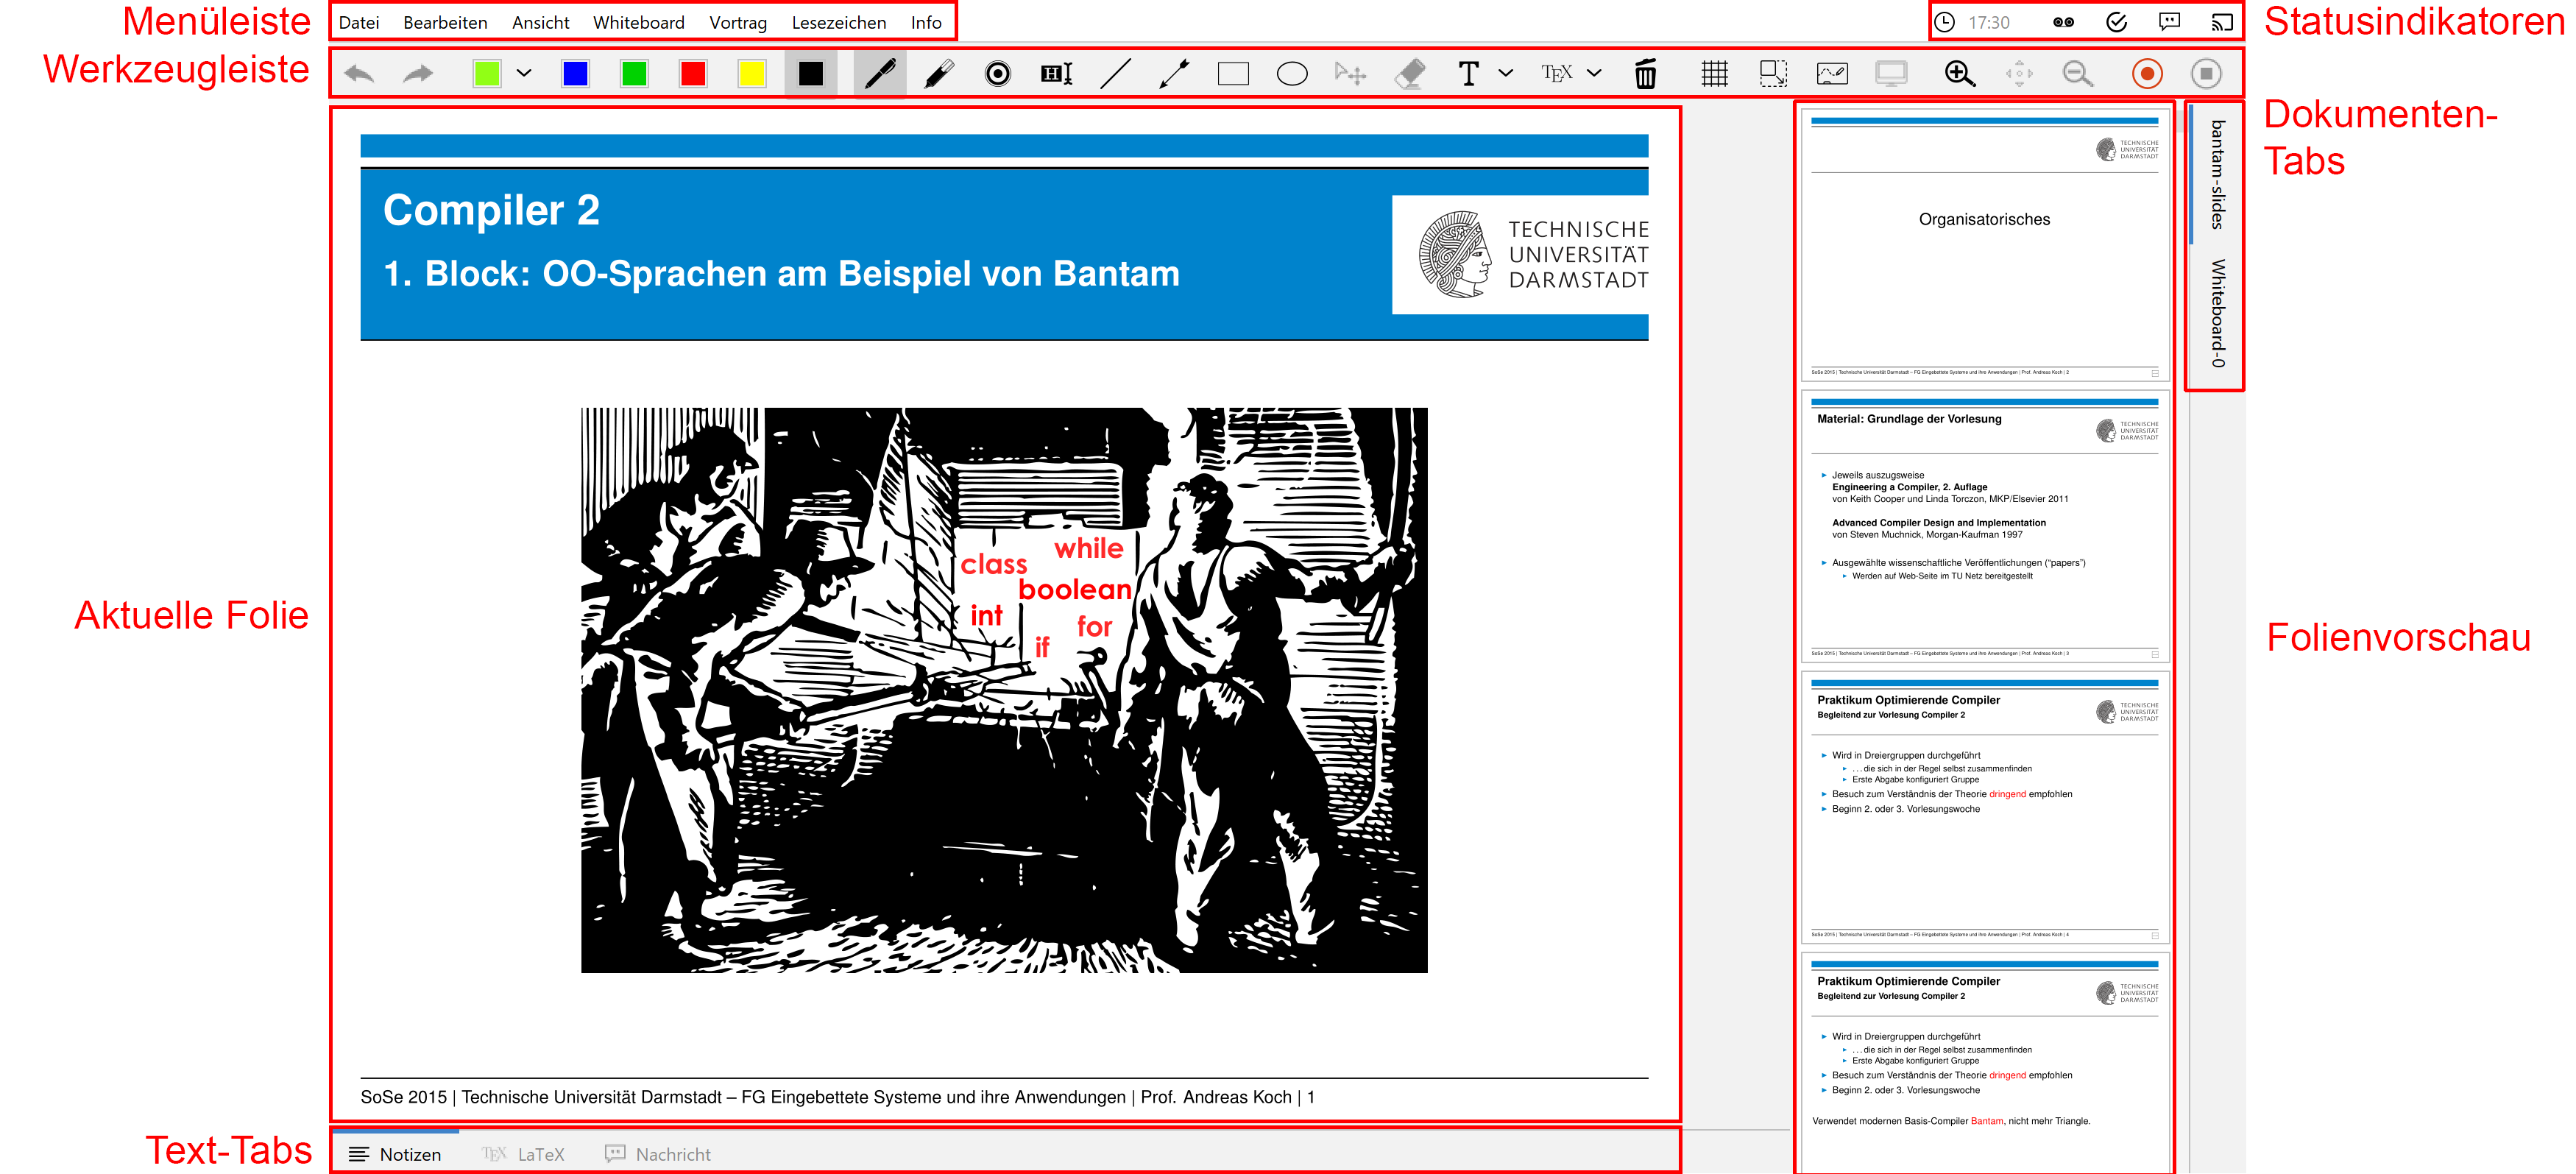
\includegraphics[width=\textwidth]{presenter/overview}
	\caption{\lectPresenter{}}
	\label{fig:presenter-overview}
\end{figure}

\subsection{Werkzeuge}
\label{section:presenter:toolbar}

\begin{figure}[H]
	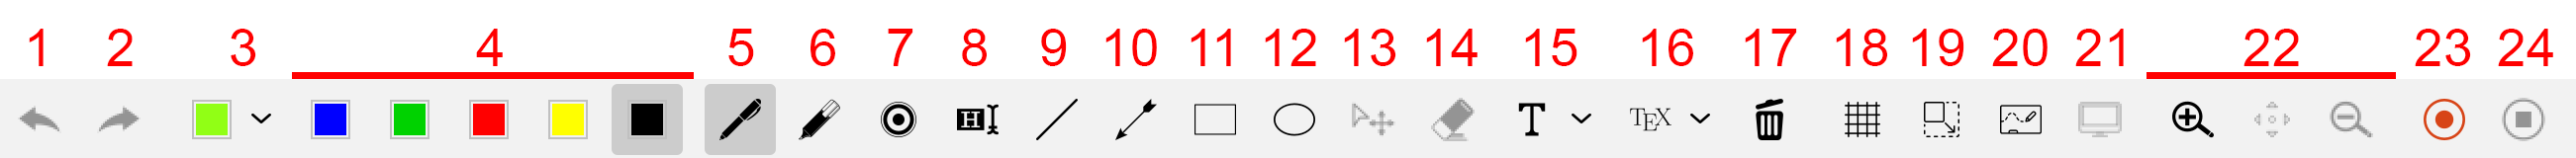
\includegraphics[width=\linewidth]{presenter/toolbar}
	\caption{\lectPresenter{}-Werkzeugleiste}
	\label{fig:presenter-toolbar}
\end{figure}

\begin{longtable}{lp{1cm}p{12cm}}
	1 &
	\begin{minipage}{.06\textwidth}
		
\includegraphics[width=\linewidth]{presenter/undo-tool}
	\end{minipage}
	& Letzte Aktion rückgängig machen. \\
	2 &
	\begin{minipage}{.06\textwidth}
		
\includegraphics[width=\linewidth]{presenter/redo-tool}
	\end{minipage}
	& Gelöschte Aktion wiederholen. \\
	3 & & Benutzerdefinierte Farbe auswählen. \\
	4 & & Vordefinierte Farben auswählen. \\
	5 &
	\begin{minipage}{.06\textwidth}
		
\includegraphics[width=\linewidth]{presenter/pen-tool}
	\end{minipage}
	& Druckempfindliche Stift-Annotation erstellen. \\
	6 &
	\begin{minipage}{.06\textwidth}
		
\includegraphics[width=\linewidth]{presenter/highlighter-tool}
	\end{minipage}
	& Highlighter-Annotation erstellen. \\
	7 &
	\begin{minipage}{.06\textwidth}
		
\includegraphics[width=\linewidth]{presenter/pointer-tool}
	\end{minipage}
	& Laserpointer-Werkzeug verwenden. \\
	8 &
	\begin{minipage}{.06\textwidth}
		
\includegraphics[width=\linewidth]{presenter/text-select-tool}
	\end{minipage}
	& Textmarker-Annotation erstellen. \\
	9 &
	\begin{minipage}{.06\textwidth}
		
\includegraphics[width=\linewidth]{presenter/line-tool}
	\end{minipage}
	& Linie erstellen. \\
	10 &
	\begin{minipage}{.06\textwidth}
		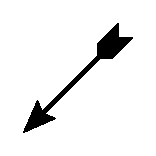
\includegraphics[width=\linewidth]{presenter/arrow-tool}
	\end{minipage}
	& Pfeil erstellen. \\
	11 &
	\begin{minipage}{.06\textwidth}
		
\includegraphics[width=\linewidth]{presenter/rectangle-tool}
	\end{minipage}
	& Rechteck erstellen. \\
	12 &
	\begin{minipage}{.06\textwidth}
		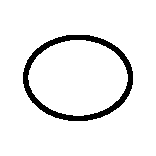
\includegraphics[width=\linewidth]{presenter/ellipse-tool}
	\end{minipage}
	& Ellipse erstellen. \\
	13 &
	\begin{minipage}{.06\textwidth}
		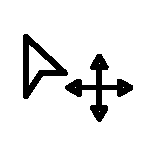
\includegraphics[width=\linewidth]{presenter/select-tool}
	\end{minipage}
	& Annotation verschieben. \\
	14 &
	\begin{minipage}{.06\textwidth}
		
\includegraphics[width=\linewidth]{presenter/rubber-tool}
	\end{minipage}
	& Ganze Annotation entfernen. \\
	15 &
	\begin{minipage}{.06\textwidth}
		
\includegraphics[width=\linewidth]{presenter/text-tool}
	\end{minipage}
	& Text erstellen. \\
	16 &
	\begin{minipage}{.06\textwidth}
		
\includegraphics[width=\linewidth]{presenter/latex-tool}
	\end{minipage}
	& LaTeX-Inhalt erstellen. \\
	17 &
	\begin{minipage}{.06\textwidth}
		
\includegraphics[width=\linewidth]{presenter/clear-tool}
	\end{minipage}
	& Alle Annotationen löschen. \\
	18 &
	\begin{minipage}{.06\textwidth}
		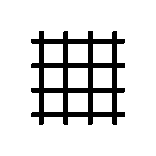
\includegraphics[width=\linewidth]{presenter/grid-tool}
	\end{minipage}
	& Gitternetz anzeigen/verstecken. \\
	19 &
	\begin{minipage}{.06\textwidth}
		
\includegraphics[width=\linewidth]{presenter/extend-tool}
	\end{minipage}
	& Zeichenbereich erweitern (verkleinert die Folie). \\
	20 &
	\begin{minipage}{.06\textwidth}
		
\includegraphics[width=\linewidth]{presenter/whiteboard-tool}
	\end{minipage}
	& Whiteboard öffnen. \\
	21 &
	\begin{minipage}{.06\textwidth}
		
\includegraphics[width=\linewidth]{presenter/display-tool}
	\end{minipage}
	& Präsentation auf angeschlossenen Bildschirmen/Projektoren anzeigen/verstecken. \\
	22 &
	\begin{minipage}{.06\textwidth}
		
\includegraphics[width=\linewidth]{presenter/zoom-in-tool}
	\end{minipage}
	& In einen Auswahlbereich reinzoomen. \\
	23 &
	\begin{minipage}{.06\textwidth}
		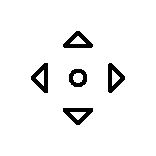
\includegraphics[width=\linewidth]{presenter/pan-tool}
	\end{minipage}
	& Gezoomte Ansicht verschieben. \\
	24 &
	\begin{minipage}{.06\textwidth}
		
\includegraphics[width=\linewidth]{presenter/zoom-out-tool}
	\end{minipage}
	& Rauszoomen in das originale Größenverhältnis. \\
	25 &
	\begin{minipage}{.06\textwidth}
		
\includegraphics[width=\linewidth]{presenter/record-tool}
	\end{minipage}
	& Aufnahme starten/pausieren. \\
	26 &
	\begin{minipage}{.06\textwidth}
		
\includegraphics[width=\linewidth]{presenter/record-stop-tool}
	\end{minipage}
	& Aufnahme beenden. \\
\end{longtable}

\subsection{Statusindikatoren}
Die dargestellten Anzeigeelemente, von links nach rechts:\\

\begin{longtable}{p{1cm}p{12cm}}
	\begin{minipage}{.05\textwidth}
		
\includegraphics[width=\linewidth]{presenter/clock-indicator}
	\end{minipage}
	& Aktuelle Uhrzeit. \\
	\begin{minipage}{.05\textwidth}
		
\includegraphics[width=\linewidth]{presenter/record-indicator}
	\end{minipage}
	& Gibt an, ob die Aufnahme gerade läuft. Orangener Hintergrund steht für \quote{pausiert}. \\
	\begin{minipage}{.05\textwidth}
		
\includegraphics[width=\linewidth]{presenter/stream-indicator}
	\end{minipage}
	& Gibt an, ob ein Echtzeit-Stream aktiv ist.. \\
	\begin{minipage}{.05\textwidth}
		
\includegraphics[width=\linewidth]{presenter/messenger-indicator}
	\end{minipage}
	& Gibt an, ob Web-Nachrichten aktiviert sind. \\
	\begin{minipage}{.05\textwidth}
		
\includegraphics[width=\linewidth]{presenter/quiz-indicator}
	\end{minipage}
	& Gibt an, ob ein Quiz aktiv ist. \\
\end{longtable}

Ist einer der Dienste aktiv, dann ist der Hintergrund des Statusindikators grau, wie z.B. bei der Aufnahme.

\begin{minipage}{\textwidth}
	\centering
	
\includegraphics[width=.5\linewidth]{presenter/indicator-active}
	\label{fig:presenter-indicator-active}
\end{minipage}


\subsection{Folienvorschau}
In diesem Bereich werden Miniaturbilder für die einzelnen Folien angezeigt. Die nächste Folie ist oben sichtbar. Um eine Folie auszuwählen, klicken Sie auf das jeweilige Miniaturbild. Beim Folienwechsel passt sich die Folienvorschau automatisch an und zeigt die nächsten Folien beginnend mit der darauffolgenden Folie von oben nach unten an. Sie haben auch die Möglichkeit das Dokument durchzublättern, indem Sie die Bildlaufleiste verwenden, um sich vorwärts und rückwärts durch das Dokument zu bewegen. Der blaue Rahmen um das Miniaturbild kennzeichnet die Folie, die gerade angezeigt wird.


\subsection{Text-Tabs}
Alle Text-Tabs sind umschaltbar, d.h. durch einen Klick auf das jeweilige Tab wird die dazugehörige Bedienoberfläche angezeigt oder versteckt.

\begin{longtable}{p{1cm}p{12cm}}
	\begin{minipage}{.05\textwidth}
		
\includegraphics[width=\linewidth]{presenter/notes}
	\end{minipage}
	& Notizen: Zeigt im Dokument eingebettete Notizen zu der aktuellen Folie an. \\
	\begin{minipage}{.05\textwidth}
		
\includegraphics[width=\linewidth]{presenter/latex-tool}
	\end{minipage}
	& LaTeX: Zeigt das Eingabefeld zum LaTeX-Werkzeug an. \\
	\begin{minipage}{.05\textwidth}
		
\includegraphics[width=\linewidth]{presenter/messenger-indicator}
	\end{minipage}
	& Nachricht: Zeigt die zuletzt eingehende Nachricht an, die über den Web-Dienst übermittelt wurde.
\end{longtable}

\section{Anwendungsszenarien}
\label{section:presenter-use-cases}
In diesem Kapitel werden häufige Anwendungsszenarien sowie deren Nutzung in \lectPresenter{} beschrieben.


\subsection{Aufnahme}
\begin{itemize}
\item \textbf{Starten Sie die Aufzeichnung!} Klicken Sie dafür auf den roten Aufnahme-Button rechts in der Werkzeugleiste (\autoref{fig:presenter-toolbar}, Markierung 23). Der \quote{Rec}-Statusindikator am oberen Bildschirmrand wechselt dann auf Grün und ein Timer erscheint links daneben.

\item Während Sie die Präsentation halten, stehen Ihnen eine Reihe von Werkzeugen zur Verfügung. Mit den Stift- und Highlighter-Werkzeugen (\autoref{fig:presenter-toolbar}, Markierungen 5 und 6) können Sie nach Belieben auf die aktuelle Folie malen, mit dem Textmarker (Markierung 8) können Sie Text hervorheben. Um die Farbe des aktuellen Werkzeugs zu verändern, können Sie entweder eine voreingestellte Farbe auswählen (Markierung 4), oder den Farbauswahl-Dialog öffnen (Markierung 3). Um alle ihre Markierungen zu entfernen, drücken Sie einfach kurz die ESC-Taste.
Eine genauere Beschreibung der Werkzeugleiste finden Sie in Abschnitt \ref{section:presenter:toolbar}.

\item Um zwischen den Folien zu wechseln, können Sie die Pfeiltasten verwenden. Um eine bestimmte Folie direkt anzuspringen, können Sie sie auch in der Vorschauleiste am rechten Bildschirmrand anklicken.

\item Mit der F8-Taste oder dem Whiteboard-Button (\autoref{fig:presenter-toolbar}, Markierung 20) können Sie ein Whiteboard öffnen. Dieses verhält sich wie ein separates Dokument, in dem Sie nach Belieben zeichnen können. Das Whiteboard kann nach der Vorlesung als ein PDF-Dokument abgespeichert werden. Um zwischen den Folien und dem Whiteboard zu wechseln, können Sie entweder die Dokument-Tabs am rechten Bildschirmrand nutzen, oder erneut die F8-Taste betätigen.

\item Die Zoom-Buttons (\autoref{fig:presenter-toolbar}, Markierung 22) können Sie verwenden, um einen Bereich der aktuellen Folie vergrößert anzuzeigen.
\end{itemize}


\subsection{Lesezeichen verwalten}
\label{section:presenter-bookmarks}
Um während der Vorlesung schnell zwischen bestimmten Folien wechseln zu können, bietet Ihnen \lectPresenter{} die Möglichkeit, Lesezeichen anzulegen und zu diesen zu springen.

\paragraph{Lesezeichen anlegen}
Um ein Lesezeichen auf der aktuellen Folie anzulegen, wählen Sie den Menüpunkt \menu[,]{Lesezeichen, Aktuelle Folie als Leerzeichen} oder drücken Sie die Taste \keys{B}. Dies öffnet die Lesezeichenliste (\autoref{fig:bookmark-set}) und fordert Sie auf, eine Tastenkombination als Shortcut festzulegen. Drücken Sie eine beliebige Taste auf der Tastatur, die Sie noch keinem Lesezeichen zugewiesen haben.

\paragraph{Lesezeichen anspringen}
Drücken Sie anschließend die Taste \keys{G} oder wählen Sie den Menüeintrag \menu[,]{Lesezeichen, Lesezeichen anspringen}, so werden Sie erneut aufgefordert, eine Tastenkombination einzugeben. Stimmt diese Kombination mit der eines zuvor zugewiesenen Lesezeichens überein, so wird die Folie unter dem entsprechenden Lesezeichen angezeigt.
\\\\
Nachdem Sie ein Lesezeichen angesprungen haben, können Sie wieder zurück zur vorherigen Folien wechseln:
\begin{itemize}
	\item Taste \keys{L}, oder
	\item Menüeintrag \menu[,]{Lesezeichen, Zurück zur letzten Position}.
\end{itemize}

\paragraph{Lesezeichen entfernen}
Um ein Lesezeichen zu löschen, gibt es mehrere Möglichkeiten:

\begin{itemize}
	\item Alle Lesezeichen löschen über Menüeintrag \\\menu[,]{Lesezeichen, Alle Lesezeichen löschen}.
	\item Lesezeichenliste mit Taste \keys{B} oder \keys{G} öffnen und auf den Button \begin{minipage}{0.025\textheight}
		
\includegraphics[width=\linewidth]{presenter/clear-tool}
	\end{minipage} neben dem Lesezeichen klicken.
\end{itemize}

\begin{minipage}{0.9\textwidth}
	\centering
	\captionsetup{type=figure}
	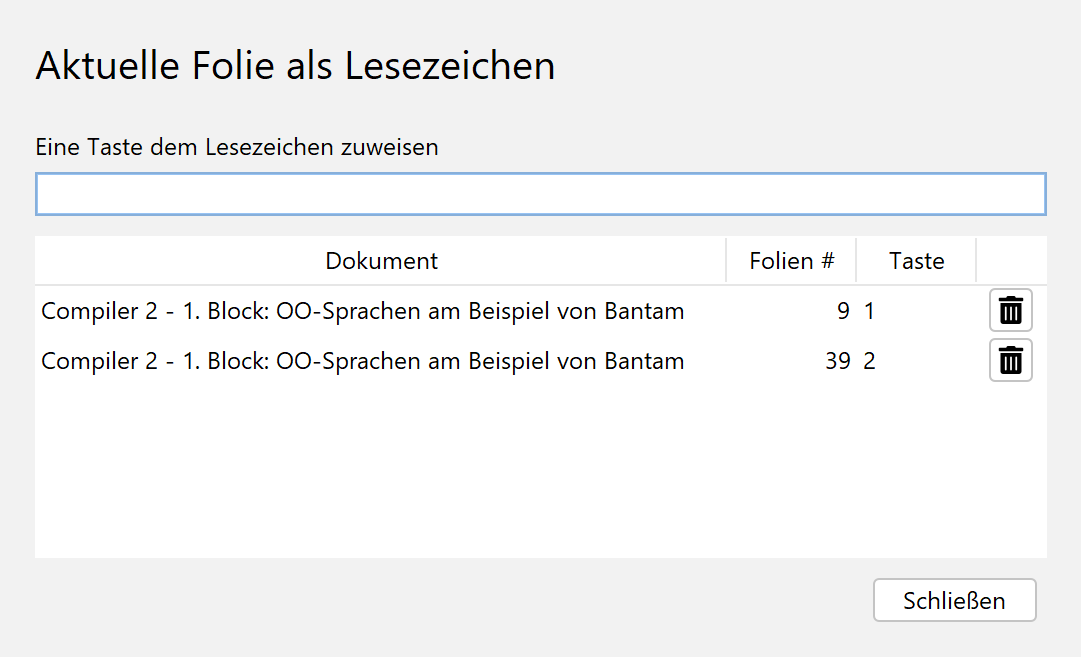
\includegraphics[width=8cm]{presenter/bookmark-set_de}
	\captionof{figure}{Lesezeichenliste}
  	\label{fig:bookmark-set}
\end{minipage}


\subsection{Quiz erstellen}
\label{section:create-quiz}
\lectPresenter{} erlaubt es Ihnen, während der Vorlesung in Echtzeit Quizze zu starten, an denen die Zuhörer über einen Browser teilnehmen können. Um ein Quiz zu erstellen, müssen Sie dieses zunächst anlegen. Wählen Sie dazu den Menüpunkt \menu[,]{Vortrag, Quiz erstellen}. Es öffnet sich eine Bedienoberfläche (\autoref{fig:create-quiz}), über die Sie das Quiz erstellen.

\begin{minipage}{0.9\textwidth}
	\centering
	\captionsetup{type=figure}
	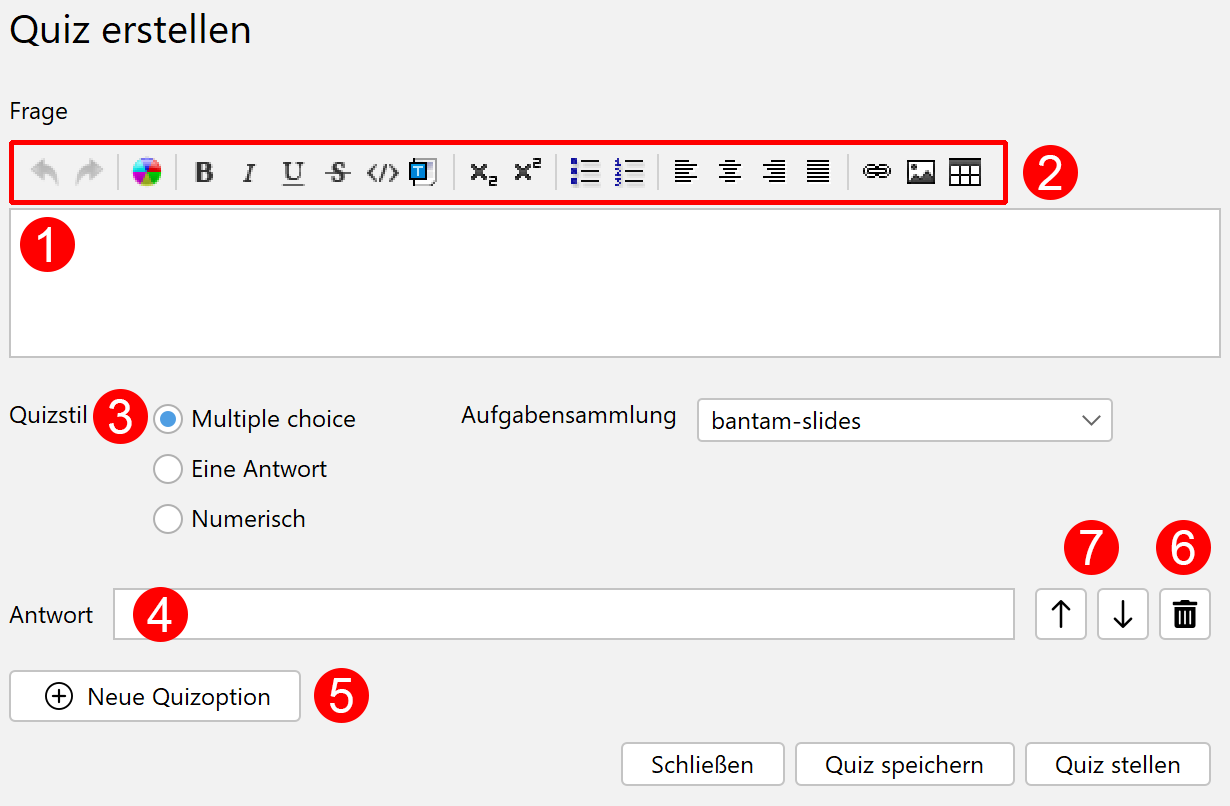
\includegraphics[width=8cm]{presenter/create-quiz_de}
	\captionof{figure}{Quiz erstellen}
  	\label{fig:create-quiz}
\end{minipage}
\\\\
Geben Sie eine Quizfrage ein [1]. Verschiedene Formatierungsmöglichkeiten sind in der Werkzeugleiste [2] zu finden. Die Quizfrage wird mit HTML formatiert. Auf diese Weise wird die Frage in allen Browsern mit der gleichen Formatierung angezeigt.
\\\\
Wählen Sie den Quizstil [3] aus. Es stehen drei Stile zur Verfügung; \quote{Multiple choice} (Mehrfachauswahl), \quote{Eine Antwort} und \quote{Numerisch}.
\\\\
\paragraph{Multiple Choice und Eine Antwort}
Die Antwortmöglichkeiten werden im Feld [4] als Text eingegeben. Neue Antwortmöglichkeiten erstellen Sie mit dem Button [5] oder mit der Taste \keys{Tab}. Um eine Antwort zu löschen, klicken Sie den \menu[,]{$\times$} Button [6]. Mit den aufwärts und abwärts Buttons [7] können Sie die Reihenfolge der Antworten verändern.

\paragraph{Numerische Antworten}
Für Fragen vom Stil \quote{Numerisch} können Sie einen oder mehrere Einträge hinzufügen. Jede Antwortmöglichkeit (\autoref{fig:numeric-quiz}) besitzt eine Beschreibung [1] und ein erlaubtes Werteintervall in Form von Min- und Max-Feldern[2][3], für die Eingabe bei der Teilnahme am Quiz. Numerische Antworten lassen sich ebenfalls sortieren und entfernen, wie im vorherigen Abschnitt beschrieben.

\begin{minipage}{0.9\textwidth}
	\centering
	\captionsetup{type=figure}
	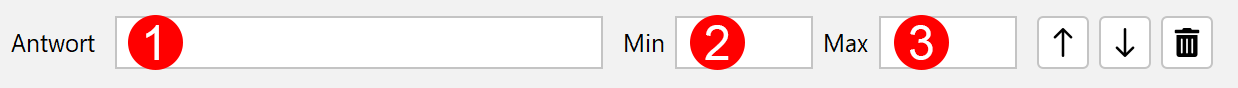
\includegraphics[width=8cm]{presenter/create-quiz-numeric_de}
	\captionof{figure}{Numerische Quizantwort}
  	\label{fig:numeric-quiz}
\end{minipage}
\\\\
Nachdem Sie alles Gewünschte eingegeben haben, haben Sie die Möglichkeit das Quiz zu speichern, bevor Sie das Quiz freigeben. Zum Speichern drücken Sie den Button \quote{Quiz speichern}. Um das Quiz freizugeben, drücken Sie den Button \quote{Quiz stellen}.
\\\\
Sobald das Quiz erfolgreich freigegeben wurde, öffnet sich ein neues Dokument mit dem Namen \quote{Quiz} und das Quiz ist jetzt für die Zuhörer über einen Browser zugänglich.
Das Quiz-Dokument wird in Echtzeit aktualisiert während die Antworten eintreffen. Um die Quizergebnisse anzuzeigen, wechseln sie auf die nächste Folie des Quiz-Dokuments.

Auf dem Projektor erscheint die IP-Adresse, unter der die Zuhörer auf das Quiz zugreifen können. Momentan sind Quizze nur über die Eingabe einer IP-Adresse in der Adressleiste des Browsers zugänglich. Wie Sie die IP-Adresse herausfinden, ist in Abschnitt \ref{section:get-ip} beschrieben.

Um das Quiz wieder zu beenden, wählen Sie den Menüpunkt \menu[,]{Vortrag, Quiz schließen}.


\subsection{Quiz aus der Quizsammlung auswählen}
\label{section:select-quiz}
Um den Zuhörern eine ihrer angelegten Fragen aus ihrer Quizsammlung zu stellen, wählen Sie den Menüpunkt \menu[,]{Vortrag, Quiz auswählen}. Es öffnet sich die Fragenliste, in der Sie bestehende Fragen bearbeiten, löschen oder stellen können. Wählen Sie die gewünschte Frage aus und klicken Sie den \textbf{Quiz stellen} Button.

\begin{minipage}{0.9\textwidth}
	\centering
	\captionsetup{type=figure}
	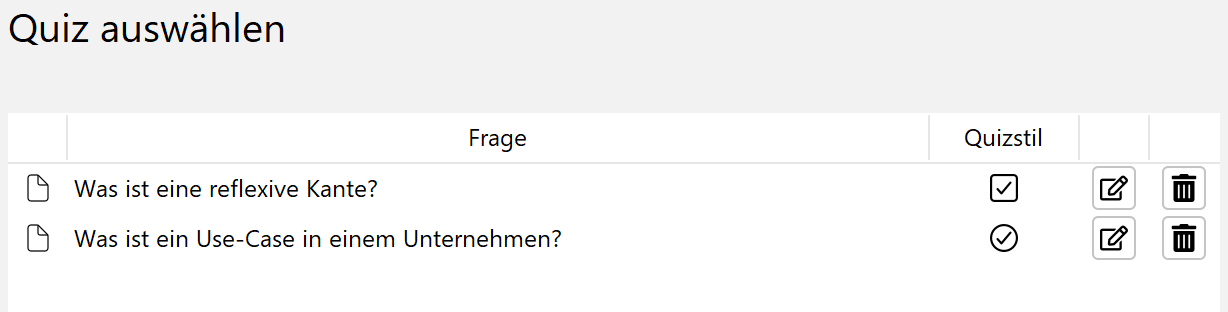
\includegraphics[width=8cm]{presenter/select-quiz_de}
	\captionof{figure}{Quiz auswählen}
  	\label{fig:select-quiz}
\end{minipage}


\subsection{Web-Nachrichten}
\label{section:web-messages}
Mit Web-Nachrichten erlauben Sie ihren Zuhörern ihnen Textnachrichten über einen Browser zu senden. Web-Nachrichten aktivieren Sie über das Menü \menu[,]{Vortrag, Messenger starten}. Dies kann einen Augenblick dauern. Während der Dienst für Web-Nachrichten gestartet wird, können Sie mit ihrem Vortrag fortfahren. Nachdem der Dienst erfolgreich gestartet ist, können die Zuhörer mittels der IP-Adresse, die auf dem externen Anzeigegerät angezeigt wird, die Webseite für Web-Nachrichten aufrufen. Ein Beispiel ist in \autoref{fig:messenger-browser} zu sehen.
\\\\
\begin{minipage}{0.9\textwidth}
	\centering
	\captionsetup{type=figure}
	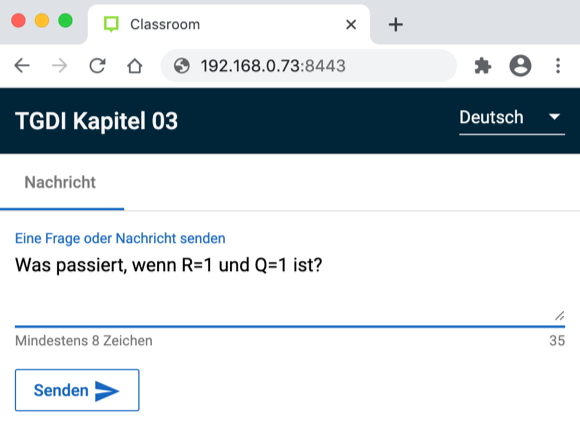
\includegraphics[width=8cm]{presenter/messenger-browser}
	\captionof{figure}{Messenger: Nachricht senden mit einem Browser}
  	\label{fig:messenger-browser}
\end{minipage}
\\\\
In \lectPresenter{} öffnet sich ein Textfeld unter der Vorschauleiste. In diesem Textfeld wird immer die zuletzt empfangene Nachricht angezeigt (\autoref{fig:messenger-presenter}).
\\\\
\begin{minipage}{0.9\textwidth}
	\centering
	\captionsetup{type=figure}
	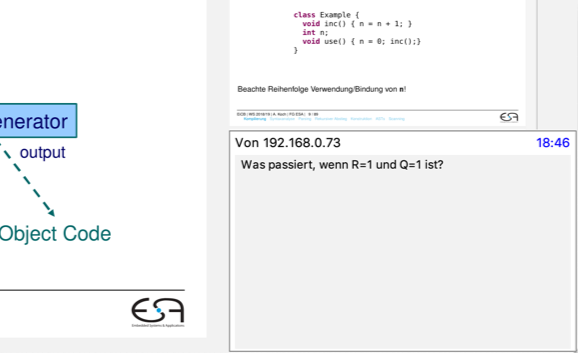
\includegraphics[width=8cm]{presenter/messenger-presenter}
	\captionof{figure}{Messenger Nachrichten in \lectPresenter}
  	\label{fig:messenger-presenter}
\end{minipage}
\\\\
Um alle Nachrichten zu lesen, öffnen Sie das Messenger-Fenster, das sich über das Menü \menu[,]{Vortrag, Messenger anzeigen} anzeigen und schließen lässt.
\\
Alle eingegangenen Web-Nachrichten werden im Ordner \inlinecode{app/AppData/Presenter} im Installationsverzeichnis in Form von einer HTML-Datei abgespeichert. Der Name der HTML-Datei trägt das Datum und die Uhrzeit zu dem der Web-Nachrichten-Dienst gestartet wurde. Es werden die IP-Adresse, Uhrzeit und die Textnachricht abgespeichert.
\\
\begin{note}
	Die Nachrichten bekommen nur Sie zu sehen!
\end{note}
\begin{info}
	Damit der Dozent seinen Vortrag nicht durch Tippen einer oder mehreren Antworten unterbricht, wird auf die bidirektionale Kommunikation mittels Web-Nachrichten verzichtet.
	
	Es besteht die Möglichkeit auf eine Nachricht verbal einzugehen oder diese zu ignorieren, wenn die Nachricht nicht zum Kontext des Vortrags passt.
\end{info}


\section{Menüs}
\subsection{Datei}
\begin{itemize}
\item \menu[,]{Öffnen}\\Öffnet den Dateiauswahldialog, über den eine Präsentation im PDF Format geladen werden kann.
\item \menu[,]{Schließen}\\Schließt die aktuell ausgewählte Datei (Auswahl über die Tabs am rechten Bildschirmrand).
\item \menu[,]{Dokumente abspeichern}\\Öffnet den Speicherdialog, über den alle geöffneten Dokumente (PDF, Whiteboard und Quizze) mitsamt aller Annotationen getrennt oder zusammen gespeichert werden können.
\item \menu[,]{Quizergebnisse abspeichern}\\Öffnet den Speicherdialog, um Quizergebnisse in Form von PDF-Diagrammen und Tabellen im CSV-Format zu speichern.
\item \menu[,]{Zuletzt geöffnete Dateien}\\Öffnet eine Liste der bis zu 5 zuletzt geöffneten Dokumente.
\item \menu[,]{Beenden}\\Beendet das Programm.
\end{itemize}
\subsection{Bearbeiten}
\begin{itemize}
\item \menu[,]{Einstellungen}\\Öffnet die Einstellungen für \lectPresenter{}.
\end{itemize}
\subsection{Ansicht}
\begin{itemize}
\item \menu[,]{Vollbild}\\Wechselt zwischen Fenster- und Vollbildmodus.
\item \menu[,]{Erweiterte Einstellungen}\\Aktiviert oder deaktiviert die Anzeige zusätzlicher Optionen in den Einstellungen.
\end{itemize}
\subsection{Whiteboard}
\begin{itemize}
\item \menu[,]{Whiteboard erstellen}\\Öffnet ein neues, leeres Whiteboard, das als Zeichenfläche genutzt werden kann.
\item \menu[,]{Whiteboardseite erstellen}\\Fügt dem aktuell geöffneten Whiteboard eine neue Seite hinzu.
\item \menu[,]{Whiteboardseite löschen}\\Löscht die aktuelle Seite des aktuellen Whiteboards.
\item \menu[,]{Gitternetz ein/ausschalten}\\Zeigt und versteckt das Gitternetz auf dem aktuellen Whiteboard.
\end{itemize}
\subsection{Vortrag}
\begin{itemize}
\item \menu[,]{Aufzeichnung starten}\\Startet die Aufzeichnung von Audio- und Zeichen-Events. Der Menüeintrag wechselt dann zu \menu[,]{Aufzeichnung pausieren}.
\item \menu[,]{Aufzeichnung stoppen}\\Beendet die Aufnahme und öffnet den \quote{Aufnahme speichern}-Dialog.
\item \menu[,]{Live-Stream starten}\\ Startet den Dienst für eine Echtzeit-Übertragung des Vortrags.
\item \menu[,]{Live-Stream stoppen}\\ Beendet die Echtzeit-Übertragung.
\item \menu[,]{Messenger starten}\\ Startet den Dienst für Web-Nachrichten.
\item \menu[,]{Messenger stoppen}\\ Beendet den Dienst für Web-Nachrichten.
\item \menu[,]{Messenger anzeigen}\\ Öffnet/schließt das Fenster, indem alle Web-Nachrichten angezeigt werden.
\item \menu[,]{Quiz auswählen}\\ Öffnet ein Dialog, in dem gespeicherte Quize aufgelistet sind.
\item \menu[,]{Quiz erstellen}\\ Öffnet ein Dialog, in dem Sie ein neues Quiz erstellen können.
\item \menu[,]{Quiz schließen}\\ Schließt das aktuelle Quiz.
\end{itemize}
\vfill

\pagebreak
\section{Tastenbelegung}
\newcommand{\altKey}{Alt}
\newcommand{\ctrlKey}{Strg}
\newcommand{\shiftKey}{Shift}

\begin{longtable}{|p{3,5cm}|l|}
	\hline
	{\ctrlKey} + O & Datei öffnen.\\
	\hline
	{\ctrlKey} + F4 & Datei schließen.\\
	\hline
	{\ctrlKey} + Q & Programm beenden.\\
	\hline
	{\altKey} + Enter & Vollbildmodus umschalten.\\
	\hline
	F9 & Whiteboardseite erstellen.\\
	\hline
	{\ctrlKey} + D & Aktuelle Whiteboardseite löschen.\\
	\hline
	Z & Quiz auswählen.\\
	\hline
	B & Lesezeichen auf die aktuelle Folie setzen.\\
	\hline
	G & Zu einem Lesezeichen springen.\\
	\hline
	L & Zur letzten Folie zurück springen.\\
	\hline
	{\ctrlKey} + Z & Letzte Aktion rückgängig machen.\\
	\hline
	{\ctrlKey} + Y & Gelöschte Aktion wiederholen.\\
	\hline
	F1 & Benutzerdefinierte Farbe auswählen.\\
	\hline
	F2 & Blaue Farbe auswählen.\\
	\hline
	F3 & Grüne Farbe auswählen.\\
	\hline
	F4 & Rote Farbe auswählen.\\
	\hline
	F5 & Gelbe Farbe auswählen.\\
	\hline
	F6 & Schwarze Farbe auswählen.\\
	\hline
	P & Druckempfindliche Stift-Annotation erstellen..\\
	\hline
	H & Highlighter-Annotation erstellen.\\
	\hline
	A & Laserpointer-Werkzeug verwenden.\\
	\hline
	S & Textmarker-Annotation erstellen.\\
	\hline
	I & Linie erstellen.\\
	\hline
	W & Pfeil erstellen.\\
	\hline
	R & Rechteck erstellen.\\
	\hline
	C & Ellipse erstellen.\\
	\hline
	O & Annotation verschieben.\\
	\hline
	E & Ganze Annotation entfernen.\\
	\hline
	T & Text erstellen.\\
	\hline
	X & LaTeX-Inhalt erzeugen.\\
	\hline
	Esc & Alle Annotationen löschen.\\
	\hline
	Q & Gitternetz anzeigen/verstecken.\\
	\hline
	F7 & Zeichenbereich erweitern (verkleinert die Folie).\\
	\hline
	F8 & Whiteboard öffnen.\\
	\hline
	F10 & In einen Auswahlbereich reinzoomen.\\
	\hline
	F11 & Gezoomte Ansicht verschieben.\\
	\hline
	F12 & Rauszoomen in das originale Größenverhältnis.\\
	\hline
	\caption{\lectPresenter{}-Tastenbelegung}
	\label{tab:shortcuts}
\end{longtable}

\pagebreak